\chapter{Nmap Port Scan Detection and Response}
\label{app:nmap-port-scan}

This appendix provides supporting evidence for the Nmap reconnaissance validation scenario summarized in Chapter~4. The objective of this scenario was to verify that SOCaaS can detect network scanning activity, enrich the resulting alert context, notify the analyst, and create an investigation trail without overloading the main implementation chapter with operational screenshots.

\begin{figure}[H]
\centering
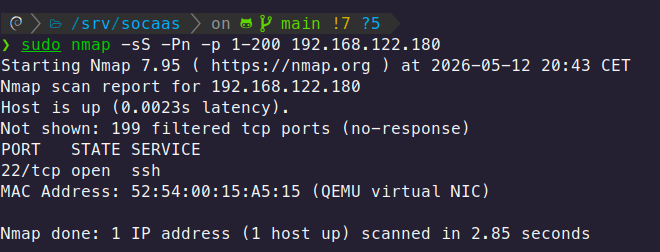
\includegraphics[width=0.90\textwidth]{figs/nmap_scan_cli.png}
\caption{Controlled Nmap Port Scan Command}
\label{fig:app-a-nmap-scan-cli}
\end{figure}

The scan was executed in the laboratory network against a monitored endpoint. The resulting telemetry was collected by the endpoint agent and evaluated by Wazuh rules before being forwarded to the SOCaaS automation pipeline.

\begin{figure}[H]
\centering
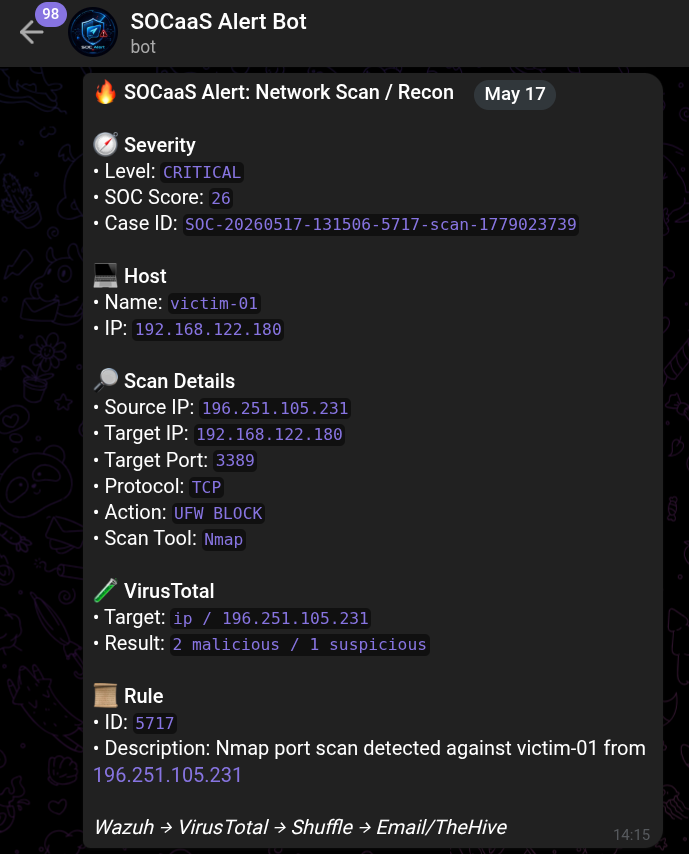
\includegraphics[width=0.55\textwidth]{figs/telegram_nmap_scan_notification.png}
\caption{Telegram Notification for Nmap Port Scan Detection}
\label{fig:ch4-telegram-nmap-scan}
\end{figure}

The Telegram notification confirms that the reconnaissance activity was converted into an analyst-facing alert. The short notification format was intentionally used for rapid awareness, while richer evidence remained available in TheHive and Shuffle execution records.

\begin{figure}[H]
\centering
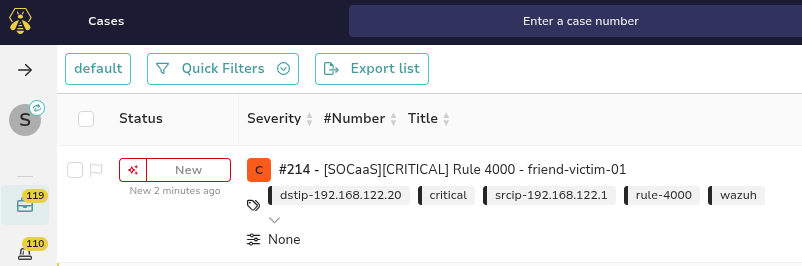
\includegraphics[width=0.90\textwidth]{figs/thehive_nmap_case_entry.png}
\caption{TheHive Case Created for Nmap Port Scan Detection}
\label{fig:app-a-thehive-nmap-case}
\end{figure}

The TheHive case preserves the investigation context for the port scan scenario, including severity, source information, and case metadata. This validates the end-to-end SOCaaS path from detection to case management for reconnaissance activity.
